\documentclass{patmorin}
\listfiles
\usepackage{amsthm,amsmath,graphicx,wrapfig}
\usepackage{pat}
%\usepackage{coffee4}
\usepackage[letterpaper]{hyperref}
\usepackage[dvipsnames]{color}
\definecolor{linkblue}{named}{Blue}
\hypersetup{colorlinks=true, linkcolor=linkblue,  anchorcolor=linkblue,
citecolor=linkblue, filecolor=linkblue, menucolor=linkblue, pagecolor=linkblue,
urlcolor=linkblue} 


\usepackage{tikz,hyphenat}
\let\oldmarginpar\marginpar
% renew the \marginpar command to draw 
% a node; it has a default setting which 
% can be overwritten
\renewcommand{\marginpar}[2][rectangle,draw,fill=yellow,rounded corners,text width=2.21cm]{%
        \oldmarginpar{%
        \tikz \node at (0,0) [#1]{#2};}%
        }
\newcommand{\note}[1]{\marginpar{\raggedright\footnotesize\nohyphens{#1}}}

\newcommand{\eps}{\varepsilon}

\title{\MakeUppercase{Dynamic Finger and Working Set: Approaching the Lower Bounds}}
\author{Luis Barba and Pat Morin}


\begin{document}
\begin{titlepage}
\maketitle
%\cofeAm{0.7}{0.38}{0}{5.5cm}{3.5in}

\begin{abstract}
  This paper begins the process of making practical comparison-based
  dictionaries that have the dynamic finger and working-set properties.
  In particular, we initiate the study of the exact number of comparisons
  needed in dynamic dictionaries that have these two properties.  We
  present a data structure with the dynamic finger property that performs
  at most $\log_2 d+o(\log d)$ comparisons per search and a data structure
  that has the working-set property and, for any $\eps > 0$, that
  performs at most $(1+\eps)\log_2 w+o(\log w)$ comparisons per search.
  Here $d$ and $w$ are the ``finger number'' and ``working-set number'',
  respectively, of the element being searched for.  All previously-known
  structures with the dynamic-finger or working-set property properties
  perform at least $2\log_2 d$ or $3\log_2 w$ comparison, respectively.
\end{abstract}

\end{titlepage}

\section{Introduction}

Comparison-based dictionaries supporting the operations
\emph{insert}, \emph{remove} and \emph{search} represent \emph{the}
classic data-structuring problem in computer science.  AVL trees, a
comparison-based asymptotically optimal solution to the dynamic dictionary
problem, were discovered already in 1962 \cite{adelsson.vleski.ea:blah}.
AVL trees implement all three operations in $O(\log n)$ time per operation
while performing at most $1.4404\log(n+2)$ comparisons between the element
being inserted/deleted/searched and the elements stored in the AVL tree.
(Here, and throughout, all logarithms are binary unless specifically
subscripted, so $\log x \equiv \log_2 x$.)

Since the discovery of AVL trees, many other comparison-based
dictionaries have been proposed: 2-3 trees \cite{X}, red-black trees
\cite{X}, splay trees \cite{X}, scapegoat trees \cite{X, Y}, skiplists
\cite{X}, treaps \cite{X,Y}, randomized binary search trees \cite{X},
and jumplists \cite{X} are just a few of the colorful names for data
structures that solve the dictionary problem in $O(\log n)$ time
per operation.\footnote{Some of these structures use amortization,
in which case the $O(\log n)$ running-time bound is only an amortized
bound.  Some of these structures use randomization, in which case the
running-time bound is an expected running time bound.}  All of these
structures perform, in the worst case, $c\log n + o(\log n)$ comparisons
per operation, for some constant $c>1$. Different structures guarantee
different upper-bounds on $c$.

\subsection{Constants}

A handful of lesser-known structures perform even fewer comparisons.
For these structures, the goal is to minimize the number of comparisons
while still supporting all operations in $O(\log n)$ time.  In their
theses \cite{X,Y} and in resulting papers, Lai and Andersson \cite{X,Y,Z}
present a series of schemes for maintaining binary search trees with
height at most $\lceil\log(n+1)\rceil+1$ in $O(\log n)$ time per insert,
update, and remove operation.  Note that $\lceil\log(n+1)\rceil$ is
a lower-bound on the height of any binary search tree containing $n$
elements, so these trees are within 1 of the minimum possible height.

Fagerberg \cite{fagerberg:complexity} tightens these results even
further by showing that, for any $c>0$, it is possible to maintain
a binary search tree with height at most $\lceil\log(n+1)+c/\log
n\rceil$ while still performing all operations in $O((1/c)\log n)$
amortized time.  This result is matched by a lower-bound: No binary
search tree that performs insertions and deletions in $O((1/c)\log n)$
time can guarantee a height smaller than $\lceil\log(n+1)+c/\log n\rceil$
\cite{fagerberg:binary-how-low-can-you-go}.  Taken together, this upper
bound and lower bound more or less close the book on the worst-case
number of comparisons achievable by comparison-based dictionaries that
support all operations in $O(\log n)$.

\subsection{Properties}

A more recent trend in the design of comparison-based dictionaries
is the study of dictionaries with special running-time \emph{properties}.
Examples include the dictionaries with 
\begin{description}
\item[the static-optimality property] in which the average access time is
   proportional to the (empirical) entropy of the distribution of
   searches;

\item[the dynamic finger property] in which the time to perform the current
   search for an element, $x$, is logarithmic in the difference in ranks between
   $x$ and the element $y$ found in the previous search; and

\item[the working-set property] in which the time to perform the current
   search for an element, $x$, is logarithmic in the number of distinct
   elements accessed since the most recent previous access to $x$.
\end{description}
There are additional properties, including the unified property
\cite{IXX}, and the dynamic optimality property \cite{X}, but the three
properties discussed above seem to be among the most fundamental.

The study of \emph{biased dictionaries}, that satisfy the
static-optimality property has a long and rich history.  A classic
result in this area is that of Mehlhorn \cite{mehlhorn:best}.
Mehlhorn's algorithm takes as input a probability distribution
$q_0,p_1,q_1,p_2,q_2,\ldots,p_n,q_n$ and a sequence of keys
$x_0=-\infty<x_1<x_2<\cdots<x_n<x_{n+1}=\infty$.  Each $p_i$
represents the probability of searching for the key $x_i$ and $q_i$
represents the probability of searching for a key in the open interval
$(x_{i},x_{i+1})$. Mehlhorn's algorithm then builds, in linear time,
a binary search tree containing $x_1,\ldots,x_n$ where the depth of
$x_i$ is at most $\log (1/p_i)+1$ and the length of the search path
for any element in the interval $(x_i,x_{i+1})$ is at most $\log
(1/q_i)+2$. With the exception of the additive constants, 1 and 2,
these bounds are essentially the best-possible.  

Several data structures are known that can provide the dynamic
finger property, including finger search trees \cite{tarjan:xxx},
splay trees \cite{S} treaps \cite{sksk}, skiplists \cite{sksk}.
See Brodal \cite{brodal:finger} for a recent survey on finger search.
In all of these structures, a finger search takes $O(\log d)$ time and
performs at most $cd$ comparisons, for some constant $c>0$.  Here $d$
is the rank difference between the element being searched for and the
previous element searched for.  The constant, $c$, varies from structure
to structure, but is at least $4$.\note{is this true?}

Similarly, several data structures are known that provide the working-set
property, including splay trees \cite{X} and several variants of Iacono's
doubly-exponential structure \cite{X}.  These structures can perform a
search for the element $x$ in $O(\log w)$ time and $cw$ comparisons,
for some constant $c>0$. Here $w$ is the number of distinct elements
accessed since the most recent previous access to $x$ (or $w=n$ if this
is the first access to $x$).  Again, the constant, $c$, varies, but is
always at least 4.

\subsection{Constants for Dynamic-Finger and Working-Set}

In order to illustrate how important leading constants are for dynamic
dictionaries, consider a binary search tree, $T$, that contains $n=10^6$
elements, and is implemented using Andersson, Lai, or Fagerberg's binary
search trees.  Such a structure can perform any search using at most
\[
   \lceil\log(10^6+1)\rceil+1= 21
\]
comparisons.  In contrast, consider storing the same elements in
a dictionary, $S$ implemented using splay trees.  The (amortized)
number of comparisons performed during a search in $S$ is $4\log w$
(see \secref{working-set}).  Thus, in order for $S$ (a splay tree)
to perform faster than $T$ (a balanced binary search tree), we must have
\[
   4\log w < 21 
       \Leftrightarrow \log w < 5.25 
       \Leftrightarrow w \le 38 \enspace .
\]
That is, of the one million elements stored in $D$ and $T$, there are
only 38 that can be accessed faster in $S$ than in $T$.  On the other
hand, the remaining $10^6 - 38$ elements require more comparison to
access in $S$ than in $T$, most by a factor of 2--4.  Furthermore, $S$
performs $3\log w$ rotations after every search, while searches do not
affect the structure of $T$ at all.  Taking all this into consideration,
it seems difficult to imagine \emph{any} realistic application where
the working-set property of splay trees would give better performance
than (Andersson, Lai, or Fagerberg's) balanced binary search trees.
(This back-of-the- envelope analysis is born out by several experimental
evaluations of splay trees \cite{X,X,X}.)

Considering the preceding, it seems that a necessary condition for a
dynamic-finger structure or a working-set structure to be practical is
that the leading constant on the number of comparisons performed during a
search should be very small, ideally this constant should be 1.  In this
paper we present two data structures that attempt to achieve this ideal.
Our first data structure supports dynamic-finger operations in $O(\log
d)$ time and performs at most $\log d+o(\log d)$ comparisons during any
operation. Our second data structure is parameterized by a parameter $\eps
>0$ and supports all operations in $O(\eps^{-1}\log w)$ time and performs
at most $(1+\eps)\log w+o(\log w)$ comparisons during any operation.
(Note that $\eps$ may even depend on $n$.)

We do not claim that this immediately implies our data structures
are practical, only that they satisfy a necessary condition
that prevents existing structures, such as splay trees, from being
practical. Nevertheless there are programming environments that tilt the
table heavily towards minimizing comparisons.  Consider, for example, the
Java Collections Framework \cite{jcf}.  In the JCF, a single comparison
between two \texttt{Integer} objects stored in a \texttt{SortedMap}
(which is implemented as a red-black tree) involves
\begin{enumerate}
\item dereferencing the data structure's \texttt{Comparator} object, \texttt{c};
\item calling \texttt{c}'s \text{compare(a,b)} method, which requires both a function call and a dereferencing operation in \texttt{c}'s dispatch table; and
\item the \texttt{compare(a,b)} method must then dereference \texttt{a} and \texttt{b}'s native variables and compare them using the \text{icmp} instruction.
\end{enumerate}
In this way, a single comparison performed within the data structure
involves a function call and four dereferencing operations, each of which
is an order of magnitude slower than the \texttt{icmp} instruction that
actually performs the comparison.  One could argue that this is a(nother)
reason not to develop software in Java, but given that there are already
3 billion devices running Java \cite{www.java.com/en/about}, it is still
a worthwhile goal to optimize algorithms for it.

\section{Background}

\subsection{Bentley and Yao's unbounded Search.}

\subsection{Unbounded Search}

\begin{thm}\thmlabel{unbounded-search}
After this, one can use a straightforward modification of Bentley
and Yao's unbounded search algorithm \cite{byXX,kXX,xxx} to find $x$
at some position $a_j$ in $\log w + O(\log\log w)$ comparisons, where
$w=|i-j|$.\footnote{Bentley and Yao actually prove the somewhat stronger
result that the number of comparisons required is at most $\log w +
\log\log w + \log\log\log w +\cdots + O(\log^* w)$.  See also, Knuth
\cite{kXX} and Beigel \cite{bXX}.}
\end{thm}

\subsection{Fagerberg's 1-2 Trees}

Fagerberg's 1-2 trees \cite{fagerberg:complexity}, maintain a 1-2 tree
of height at most $\log n +O(1)$, support insertion and deletion, and
have an amortized rebalancing cost of $O(1)$ per update.  We modify this
data structure slightly so that all keys are stored in the leaves. Each
internal node, $u$, stores a value that upper-bounds the largest value
stored at any leaf in $u$'s subtree. However, this value never exceeds the
smallest value stored in any leaf to the right of $u$'s subtree\ldots




\section{The Dynamic-Finger Property}

We begin this section by observing that, in the absence of insert or
remove operations, the dynamic-finger property is easy to achieve simply
by storing the data in a sorted array, $A=a_1,\ldots,a_n$, and maintaining
the index, $i$, of the most recently accessed element.  When searching
an element $x$, a single comparison suffices to determine if the search
should proceed in $a_i,\ldots, a_n$ or in $a_{i-1},\ldots,a_1$ after which
one can apply \thmref{unbounded-search} to find $x$ in $O(\log x)$ time.

To obtain an efficient dynamic-finger data structure that supports insert
and delete operations, we make use of Fagerberg's 1-2 trees.




\section{The Working-Set Property}

\section{Discussion}

\subsection{Two-Way Comparisons}

\subsection{Handling Searches for Missing Values}

\section*{Acknowledgement}

The authors of this paper are partly funded by NSERC and CFI.

\bibliographystyle{abbrvurl}
\bibliography{avgstretch}

\newpage

\section*{Authors}

\noindent
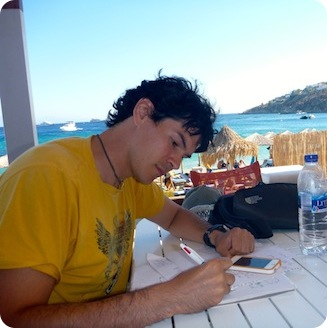
\includegraphics[width=.475\textwidth]{luis-b}% 
\hspace{.1\textwidth}%
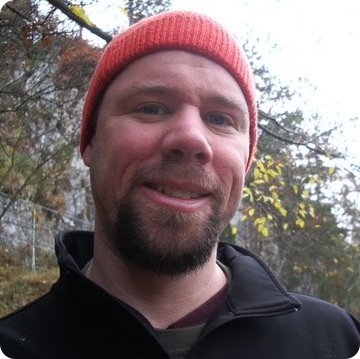
\includegraphics[width=.475\textwidth]{pat-b}%

\noindent\emph{Luis Barba.}
School of Computer Science, Carleton University, and D\'epartement
D'Informatique, Universit\'e Libre de Bruxelles

\noindent\emph{Pat Morin.}
School of Computer Scence, Carleton University

\end{document}


